\documentclass[11pt, a4paper]{article}
\usepackage{fullpage}
\usepackage[T1]{fontenc}

\usepackage{amsmath}
\usepackage{amssymb}
\usepackage[colorlinks=true, citecolor=blue, linkcolor=black]{hyperref}
\usepackage{listings}
\usepackage{xcolor}
\usepackage{graphicx}
\usepackage{caption}
\usepackage{subcaption}

\renewcommand{\figurename}{Fig.}
\renewcommand{\lstlistingname}{Algorithm}

\lstset{language=C++,
				backgroundcolor=\color{black!5},
                basicstyle=\scriptsize ,
                keywordstyle=\color{blue}\ttfamily,
                stringstyle=\color{red}\ttfamily,
                commentstyle=\color{green}\ttfamily,
                morecomment=[l][\color{magenta}]{\#},
                tabsize = 1,
}

\newcommand{\SL}{Schr\"{o}dinger }
\newcommand{\A}{\mathbf{A}}
\renewcommand{\S}{\mathbf{S}}
\newcommand{\B}{\mathbf{B}}
\newcommand{\x}{\mathbf{x}}

\title{Using Jacobi's Rotation Algorithm to Solve the Two Electron \SL Equation.}
\date{October 5, 2014}
\author{Ole Gunnar Johansen}

\begin{document}
	\maketitle
	
	\begin{abstract}
		In this project, I have implemented the Jacobi rotation algorithm to look at the eigenstates of one and two electrons in the harmonic oscillator potential. I have found that the eigenvalues for the three lowest states to a very high precision. In the one electron case, they were found to be $\lambda_1 = 2.999$, $\lambda_2 = 6.999$ and $\lambda_3 = 10.997$ compared to the analytical 3, 7 and 11 respectively.
		
		There is also made a discussion of the speed of the algorithm compared to other methods, and in relation, pros and cons connected with the Jacobi method compared to one other method. The main idea here is that the Jacobi method is intrinsically  slow, but easy to parallelize. 
		
		The source code for this project can be found at my github\footnote{\url{https://github.com/olegjo/FYS3150-project-2}}.
	\end{abstract}
	
	\section{Introduction}
		Eigenvalue problems are of great importance in the modern sciences. One such example is the \SL equation in quantum mechanics. The problem we are facing is, however, that such problems have analytical solutions only to a very small number of cases. In this project, I will solve the radial part of the \SL equation for one and two electrons in a harmonic oscillator potential with and without repulsive Coulomb interaction using the Jacobi's rotation method for finding eigenvalues.
		
		The report will be naturally structured into the one electron case and the two electron case, and additional results and discussions specific to the Jacobi method as separate sub sections.

	
	\section{Method}
		\subsection{Jacobi's rotation algorithm}
		\label{subsec: jacobi algo}
			The aim of this method is to transform a general, symmetric, $n\times n$ matrix $\A$ into a diagonal matrix $\mathbf{D}$ through a series of similarity transforms. A similarity matrix $\S$ has the property that, when used in a similarity transform on $\A$, the similar matrix $\B$ has the same eigenvalues as $\A$. A similarity transform is defined as
			\begin{align*}
				\B = \S^T \A \S
			\end{align*}
			where we require $\S^T\S = \S^{-1}\S = \mathbf{I}$. It is clear then, that this has the same eigenvalues as $\A$:
			\begin{align*}
				\A \x &= \lambda \x \\
				(\S^T\A \S)(\S^T\x) &= \lambda S^T\x \\
				\B \S^T \x &= \lambda \S^T \x 
			\end{align*}
			
			In Jacobi's rotation method, the similarity matrix $\S$ is defined as
			\begin{align*}
				\S = \begin{pmatrix} \mathbf{ I } &  &  &  & \mathbf{ 0 } \\  & \cos  \theta  & \cdots  & \sin  \theta  &  \\  & \vdots & \ddots  & \vdots  &  \\  & -\sin  \theta  & \cdots  & \cos  \theta  &  \\ \mathbf{ 0 } &  &  &  & \mathbf{ I } \end{pmatrix}
			\end{align*}
			i.e.  the $n\times n$ identity matrix with the elements $s_{kk}$, $s_{ll}$, $s_{kl}$ and $s_{lk}$ changed so that
			\begin{align*}
				s_{kk} = s_{ll} = \cos\theta, \ s_{kl} = -\sin\theta \ \mathrm{and} \ s_{lk} = \sin\theta
			\end{align*}
			where the angle of rotation $\theta$ can be chosen arbitrarily.
			The similarity transform $\B=\S^T\A\S$ then results in 
			\begin{align*}
				b_{ii} 	&= a_{ii}, \ i \neq k, \ i \neq l \\
				b_{ik} 	&= a_{ik}\cos \theta - a_{il}\sin\theta,\ i \neq k, \ i \neq l \\
				b_{il} 	&= a_{il} \cos\theta + a_{ik}\sin\theta, \ i \neq k, \ i \neq l \\
				b_{kk} 	&= a_{kk}\cos^2\theta - 2a_{kl}\cos\theta \sin\theta + a_{ll}\sin^2\theta \\
				b_{ll} 	&= a_{ll}\cos^2\theta +2a_{kl}\cos\theta\sin\theta + a_{kk}\sin^2\theta \\
				b_{kl} 	&= (a_{kk} - a_{ll})\cos\theta \sin\theta +a_{kl}(\cos^2\theta - \sin^2\theta)
			\end{align*}
			The algorithm is then, for each iteration: find the largest off-diagonal value in $\A$, $a_{kl}$. Choose the angle $\theta$ so that the non-diagonal element in the similarity matrix $b_{kl}=0$. Defining $t=\tan\theta = s/c$, $\tau=(a_{ll}-a_{kk})/2a_{kl}$, $c=\cos \theta$ and $s=\sin \theta$, the last expression above becomes 
			\begin{align*}
				(a_{kk} - a_{ll})c s +a_{kl}(c^2 - s^2) 	&= 0 \\
				 (a_{kk} - a_{ll})t + a_{kl}(1-t^2)				&= 0 \\
				 t^2 + 2\tau t - 1 &= 0 \\
				 \Rightarrow t = -\tau \pm \sqrt{1+\tau^2}
			\end{align*}
			where, in turn, the values of $\cos \theta$ and $\sin \theta$ are obtained through
			\begin{align*}
				c = \frac{1}{\sqrt{1+t^2}} \qquad \mathrm{and} \qquad s = tc
			\end{align*}
			
			Note that we have two options in the choice of two values for $t$. To see which one is the best, we need to look back at the element definitions in the matrix $\B$ above. There are three expressions which describe the change in the non-diagonal matrix elements. These are for $b_{ik}$, $b_{il}$ and $b_{kl}$, where the last is set to zero in the algorithm. After a number of similarity transforms, the elements $b_{ik}$, $b_{il}$ should approach zero. If these are sufficiently close to zero, we wish not to change them, however, we do not have a choice. We can, however, make the change as small as possible by forcing $cos\theta \rightarrow 1$ and $\sin \theta \rightarrow 0$ simultaneously - a result obtained by letting the angle $\theta$ be as small as possible.
			Therefore, by choosing the smaller of the roots for $t$, we get the least difference in these elements and convergence of the method is ensured to happen faster.
			
			When all the non-diagonal matrix elements are sufficiently close to zero, the eigenvalues of matrix $\A$ is listed along the diagonal.
			
		\subsection{Eigenvectors}
			The eigenvalues for the matrix is found using Jacobi's rotation algorithm as discussed above. The eigenvectors, however, is not returned by this method.
			
			Recall the definition of similarity transform on the system:
			\begin{align*}
				\B(\S^T\mathbf{u}_1) = \lambda_1 (\S^T\mathbf{u}_1)
			\end{align*}
			so, after a similarity transform, the similar matrix $\B$, whose eigenvalues are the same as $\A$, have the eigenvector $\S^T\mathbf{u}_1$ where $\mathbf{u}_1$ is the eigenvector of $\A$ associated with the eigenvalue $\lambda_1$. If $\B$ was a diagonal matrix, it's eigenvector would be the vectors $\mathbf{e_i}$. In this case, we would simply compute $\mathbf{u}_i = \S \mathbf{e}_i$. If we start with $\mathbf{R}=\mathbf{I}$, the unit matrix, the algorithm for iteratively approaching the eigenvectors is
			\begin{align*}
				r_{ik} &= r_{ik}\cos \theta - r_{il}\sin \theta \\
				r_{il} &= r_{il}\cos \theta + r_{ik}\sin \theta
			\end{align*}
		
		
		\subsection{Single electron \SL equation}
			The radial part of the \SL equation for one electron is
			\begin{align}
			-\frac{\hbar^2}{2m} \left( \frac{1}{r^2} \frac{d}{dr} r^2 \frac{d}{dr}-\frac{l(l + 1)}{r^2} \right) R(r) + V(r)R(r) = ER(r) \label{eq: SL one electron, normal}
			\end{align}
			we are interested in the solution in a harmonic oscillator potential, so $V(r) = (1/2)kr^2$ where $k=m\omega^2$ and $E$ is the energy of the harmonic oscillator in three dimensions. $\omega$ is the oscillator frequency and the energies can be found analytically:
			\begin{align*}
				E_{nl} = \hbar \omega \left( 2n+l+\frac{3}{2} \right) 
			\end{align*}
			with $n=0, 1, 2, ...$ and $l = 0, 1, 2, ..., n-1$. 
			
			We will substitute $R(r) = (1/r)u(r)$ and rewrite eq.~\eqref{eq: SL one electron, normal} as follows
			\begin{align*}
				-\frac{\hbar^2}{2m} \frac{d^2}{dr^2}u(r) + \left( V(r) + \frac{l(l+1)}{r^2}\frac{\hbar^2}{2m} \right) u(r) = Eu(r)
			\end{align*}
			Next, introduce a dimensionless variable $\rho = (1/\alpha)r$ where $\alpha$ is a constant with dimension length and $\rho \in [0, \infty)$. We will only be looking at solutions where $l=0$. Inserting this and $V(\rho)=(1/2)k\alpha^2\rho^2$ we get 
			\begin{align}
				-\frac{\hbar^2}{2m\alpha^2}\frac{d^2}{d\rho^2}u(\rho) + \frac{k}{2}\alpha^2\rho^2u(\rho) = Eu(\rho) \label{eq: SL one electron halfway there}
			\end{align}
			Further simplification by multiplying through by $2m\alpha^2/\hbar^2$ and fixing $\alpha$ so that
			\begin{align*}
				\frac{mk}{\hbar^2}\alpha^4 = 1
			\end{align*}
			results finally in
			\begin{align}
				-\frac{d^2}{d\rho^2}u(\rho) + \rho^2u(\rho) = \lambda u(\rho) \label{eq: SL one electron, simple}
			\end{align}
			where 
			\begin{align*}
				\lambda = \frac{2m\alpha^2}{\hbar^2}E
			\end{align*}
			which in three dimensions can take the values $\lambda_0 = 3$, $\lambda_1 = 7$, $\lambda_2 = 11$, ....
			
			Numerically, the second derivative in eq.~\eqref{eq: SL one electron, simple} can be approximated using
			\begin{align}
				\frac{d^2u(\rho)}{d\rho^2} = \frac{u(\rho + h - 2u(\rho) + u(\rho - h)}{h^2} + O(h^2) \label{eq: def. second derivative}
			\end{align}
			The variable $\rho$ can be interpreted as a distance from the center and $u(\rho)^2$ as the probability of finding the electron at the distance $\rho$. As $\rho$ increases, this probability decreases rapidly, and so, although the boundary conditions require $u(0)=0$ and $u(\infty)=0$, we can safely truncate $\rho$ to a finite number, as long as $u(\rho)$ is sufficiently small. The step length can then be defined as
			\begin{align*}
				h = \frac{\rho_\mathrm{min} - \rho_\mathrm{max}}{n}
			\end{align*}
			where $n$ is the number of steps we wish to take and $\rho_i = \rho_\mathrm{min} + ih$ for $i=0, 1, 2, ..., n$.
			
			Rewriting eq.~\ref{eq: def. second derivative} in a more compact way and inserting into eq.~\ref{eq: SL one electron, simple}, we obtain
			\begin{align*}
				-\frac{u_{i+1} - 2u_i + u_{i-1}}{h^2} + \rho_i^2u_i = \lambda u_i
			\end{align*}
			where $\rho_i^2=V_i$ is the harmonic oscillator potential.
			
			We can rewrite this as the matrix equation
			\begin{align}
			 	\begin{pmatrix} d_1 		& e_1 	& 0   	& 0    	& \dots  	&0     								& 0 \\
                                			e_1 		& d_2 	& e_2 	& 0    	& \dots  	&0     								&0 \\
                               	 		0   		& e_2 	& d_3 	& e_3  	&0       		&\dots 								& 0\\
                                			\dots  	& \dots 	& \dots 	& \dots	&\dots     	&\dots	 							& \dots\\
                                			0   		& \dots 	& \dots 	& \dots 	&\dots      	&d_{n_{\mathrm{step}}-2}	& e_{n_{\mathrm{step}}-1}\\
                                			0   		& \dots 	& \dots 	& \dots 	&\dots      	&e_{n_{\mathrm{step}}-1}	& d_{n_{\mathrm{step}}-1}
            		\end{pmatrix}        
            		\begin{pmatrix} 	u_{1} \\
                                            	u_{2} \\
                                          	\dots \\
                                          	\dots \\ 
                                          	\dots \\
                                            	u_{n_{\mathrm{step}}-1}
             	\end{pmatrix}
             	=\lambda
             	\begin{pmatrix} 	u_{1} \\
                                           	u_{2} \\
                                            	\dots \\ 
                                            	\dots \\ 
                                            	\dots\\
                             				u_{n_{\mathrm{step}}-1}
            		\end{pmatrix} 
      \label{eq: matrix eigenvalue equation}
      \end{align}
      where the diagonal matrix elements are defines as
		\begin{align*}
			d_i = \frac{2}{h^2} + V_i
		\end{align*}
		and the non-diagonal elements are
		\begin{align*}
			e_i = -\frac{1}{h^2}
		\end{align*}
	
		\subsection{Two electron \SL equation}
			Quite analogous to the one electron solution, the radial part of the \SL equation for two electrons is just the sum of the single electron solution
			\begin{align*}
				\left( -\frac{\hbar^2}{2m}\frac{d^2}{dr_1^2} - \frac{\hbar^2}{2m}\frac{d^2}{dr_2^2} + \frac{1}{2}kr_1^2 ++ \frac{1}{2}kr_2^2 \right) u(r_1,r_2) = E^{(2)}u_(r_1, r_2)
			\end{align*}		
			where $E^{(2)}$ denotes the energy for two electrons. Introducing the relative coorsinate $\mathbf{r} = \mathbf{r}_1 - \mathbf{r}_2$ and the center of mass coordinate $\mathbf{R}=(1/2)(\mathbf{r}_1+\mathbf{r}_2)$ we can rewrite the last expression as
			\begin{align*}
				\left( -\frac{\hbar^2}{m}\frac{d^2}{dr^2} - \frac{\hbar^2}{4m}\frac{d^2}{dR^2} + \frac{1}{4}kr^2 + kR^2 \right) u(r, R) = E^{(2)}u(r,R)
			\end{align*}
			Furthermore, we can perform a separation of variables on the wavefunction letting $u(r, R) = \psi(r)\phi(R)$ and the energy is given by
			\begin{align*}
				E^{(2)} = E_r + E_R
			\end{align*}
			The repulsive Coulomb interaction between two electrons is
			\begin{align*}
				V(r_1, r_2) = \frac{\beta e^2}{|\mathbf{r}_1-\mathbf{r}_2|} = \frac{\beta e^2}{r}
			\end{align*}									
			where $\beta e^2 = 1.44 \ \mathrm{eV nm}$. We can then simplify further, obtaining
			\begin{align*}
				\left( -\frac{\hbar^2}{m}\frac{d^2}{dr^2} + \frac{1}{4}kr^2 + \frac{\beta e^2}{r} \right) \psi(r) = E_r\psi(r)
			\end{align*}
			which is very similar to that in eq.~\eqref{eq: SL one electron halfway there}. Following a much similar approach as above, we obtain finally
			\begin{align}
				-\frac{d^2}{d\rho^2}\psi(\rho) + \omega_r^2 \rho^2 \psi(\rho) + \frac{1}{\rho} = \lambda \psi (\rho) \label{eq: SL two electrons simple}
			\end{align}
			where now $\rho = r/\alpha$, $\alpha$ is fixed so that
			\begin{align*}
				\frac{m\alpha \beta e^2}{\hbar^2} = 1
			\end{align*}
			$\omega_r$ can be interpreted as a frequency of the harmonic oscillator:
			\begin{align*}
				\omega_r^2 = \frac{1}{4}\frac{mk}{\hbar^2}\alpha^4
			\end{align*}
			and finally
			\begin{align*}
				\lambda = \frac{m\alpha^2}{\hbar^2}E
			\end{align*}
			
			Comparing eq.~\eqref{eq: SL one electron, simple} and eq.~\eqref{eq: SL two electrons simple}, we see that they are equal, but with the potential changing from $V_i = \rho_i^2$ to $V_i = \omega_r^2 \rho_i^2 + 1/\rho_i$.
		
	
	
		\subsection{Implementation}
			I have implemented the above methods in the C++ programming language. Note that the values for the potential in both cases are known at $i=0$ and $i=n$, namely $V_0=0$ and $V_n=0$. To create the matrix in eq.~\eqref{eq: matrix eigenvalue equation}, we therefore only need values for $\rho_i$ for $i=1,2,...,n-1$, which are plugged into the diagonal elements $d_i$. 
			
			Also, since only some elements in the matrix will change for each iteration, we need not create a new matrix, but rather change the existing matrix in place.	The implemented Jacobi is
			\begin{lstlisting}[caption=Jacobi algorithm]
int jacobi_method(double **A, double **R, int n)
{
    int iterations = 0;
    int k, l;
    double eps = 1.0e-8;
    double max_off = max_off_diag(A, &k, &l, n);
    double max_number_iterations = (double) n * (double) n * (double) n;
    while (max_off*max_off > eps && (double) iterations < max_number_iterations) {
        rotate(A, R, k, l, n);
        max_off = max_off_diag(A, &k, &l, n);
        iterations++;
    }
    return iterations;
}
			\end{lstlisting}
		
			where the function \texttt{rotate} follows the rotation algorithm presented in section~\ref{subsec: jacobi algo}. The function \texttt{max\_off\_diag} finds and returns the largest element in the current matrix $\A$, also changing the values of $k$ and $l$ so that these refer to the largest element in $\A$.

	\section{Results}
		\subsection{One electron}
			Fig.~\ref{fig: one electron P-distribution} shows the eigenstates of the electron plotted as a probability distribution as a function of $\rho$. The respective eigenvalues are indicated, and resemble those found theoretically, building confidence in the reliability of the program. As previously discussed, the value of $\rho_\mathrm{max}$ should, ideally, be $\infty$, but as fig.~\ref{fig: one electron P-distribution} shows, the probability of finding the electron outside of $\rho_\mathrm{max}\approx 5$ is almost, or equal to, zero for the three lowest eigenstates. One can therefore increase the accuracy by setting $\rho_\mathrm{max}$ lower, without needing to increase the number of grid points. Table~\ref{table: eigenvalues and rho_max} shows such a relation. Note that decreasing $\rho_\mathrm{max}$ into an area where there is a larger than zero probability of finding the electron ($\rho_\mathrm{max}<\sim 4$, has the effect of decreasing the accuracy. 
			
			\begin{figure}
				\centering
				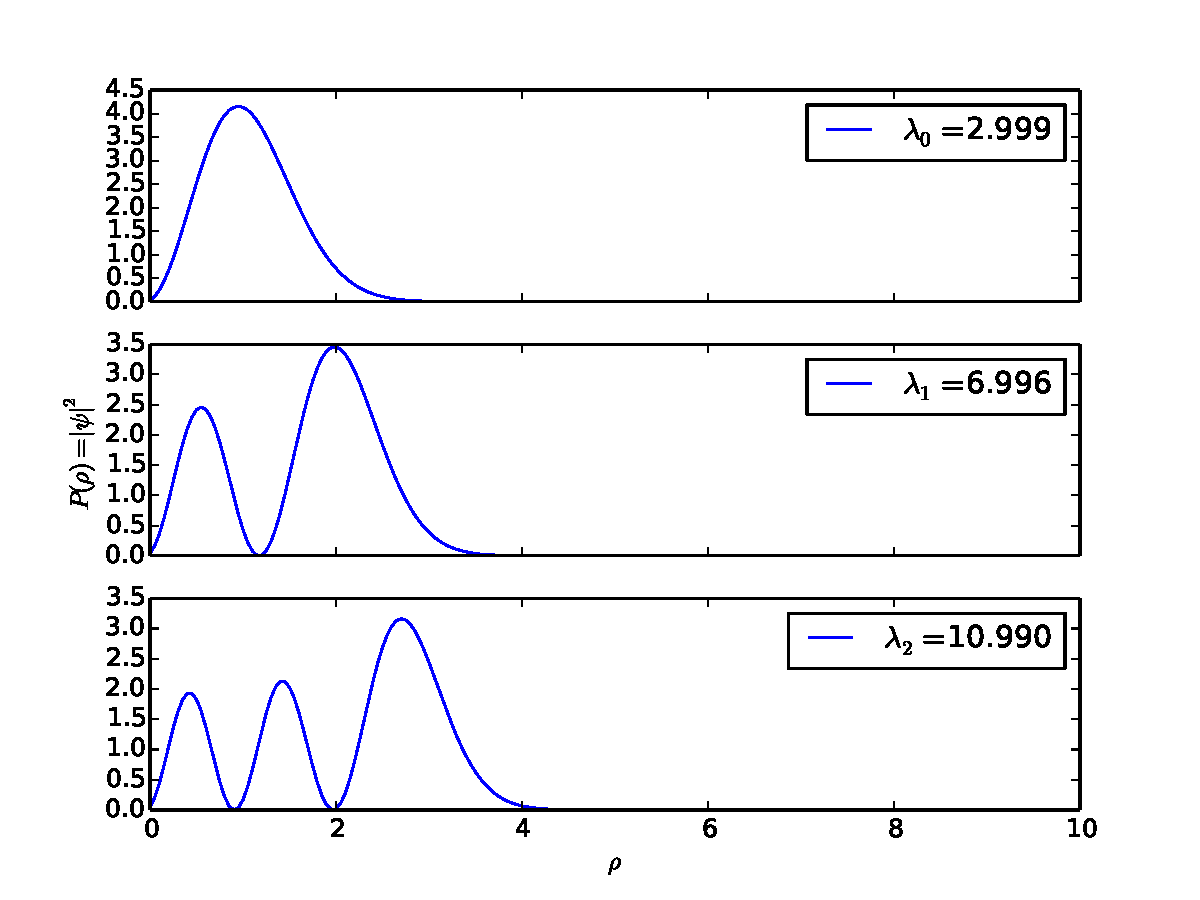
\includegraphics[scale=0.7, clip=true, trim= 0 0 0 0]{plot-oneElectron}
				\caption{Probability distribution of the eigenstates for one electron in the harmonic oscillator potential. As we can see, the eigenvalues are not completely equal the theoretical results. In this example, $n=200$ grip points and $\rho_\mathrm{max}=10$ were used.} 
				\label{fig: one electron P-distribution}
			\end{figure}
			\begin{table}
				\centering
				\caption{The accuracy of $\lambda$ increases as the density of grid points increases, here represented by decreasing values of $\rho_\mathrm{max}$. $n=200$.}
				\label{table: eigenvalues and rho_max}
				\begin{tabular}{|c|c|c|c|}
					\hline
					$\rho_\mathrm{max}$		&	$\lambda_1$	&	$\lambda_2$	&	$\lambda_3$	\\
					\hline
					10										&	2.999				&	6.996				&	10.990				\\
					8										&	2.999				&	6.997				&	10.993				\\
					6										&	2.999				&	6.998				&	10.996				\\
					5										&	2.999				&	6.999				&	10.997				\\
					4										&	2.999				&	7.002				&	11.070				\\
					\hline
				\end{tabular}
			\end{table}
			
			By the method of trial and error, it was found that $n=220$ is enough to get the three first eigenvalues stable to four leading digits.
			
			It is also of interest to find the number of transformations needed as a function of the number of grid points. Fig.~\ref{fig: number of iterations vs number og grid points} shows such a relation, and it is evident that the number of iterations needed goes like $\sim O(n^2)$, at least for $n<\sim400$. 
				\begin{figure}
					\centering
					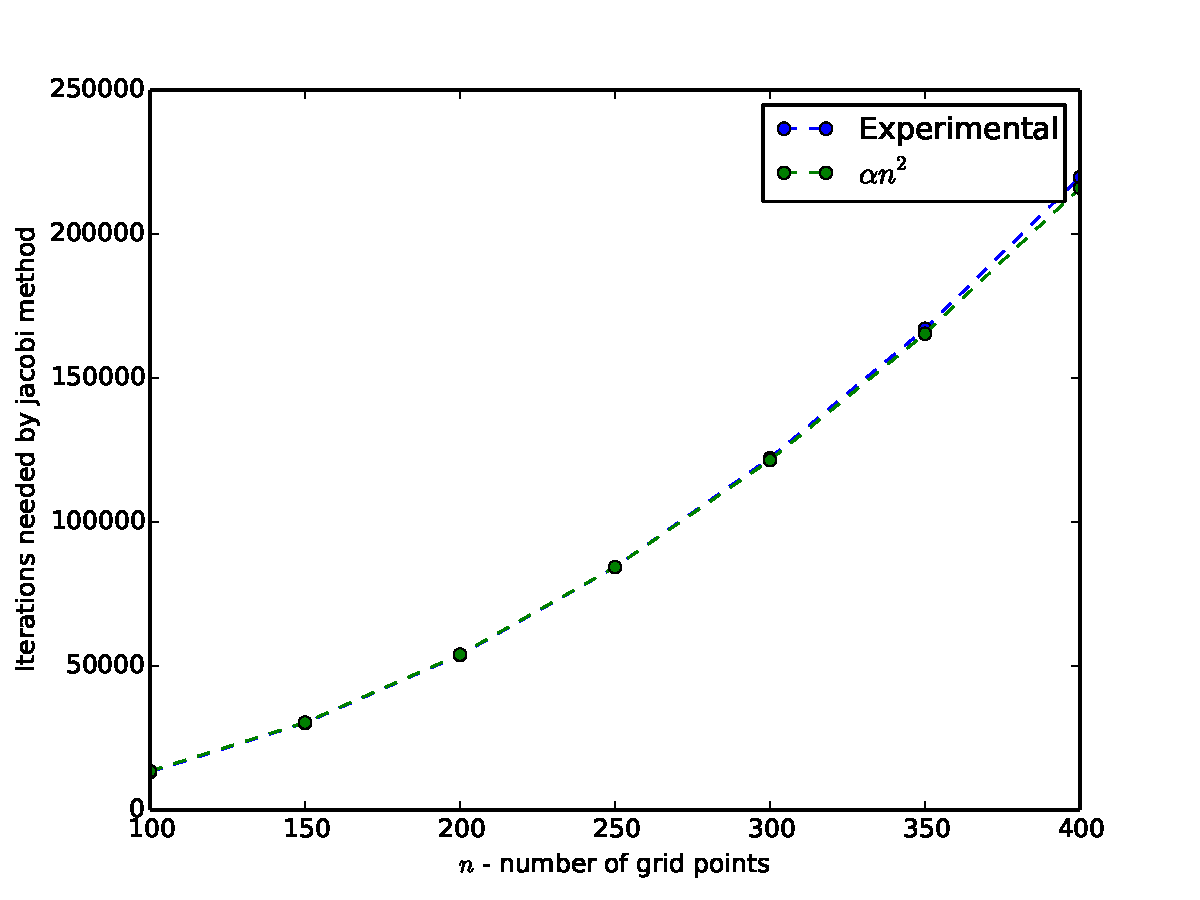
\includegraphics[scale=0.7, clip=true, trim= 0 0 0 0]{plot-grid-pointsVSiterations}
					\caption{The number iterations needed to reach diagonality of the matrix $\A$ as a function of number of grid points $n$.}
					\label{fig: number of iterations vs number og grid points}
				\end{figure}
				
		
		\subsection{Two electrons}
			For the case of two electrons, we are interested in the wavefunction for the ground state (lowest eigenvalue) for four different values of the oscillator "frequency" $\omega_r$. The results are shown in fig.~\ref{fig: plot two electrons}.
			
			\begin{figure}
				\centering
   				\begin{subfigure}[b]{0.45\textwidth}
					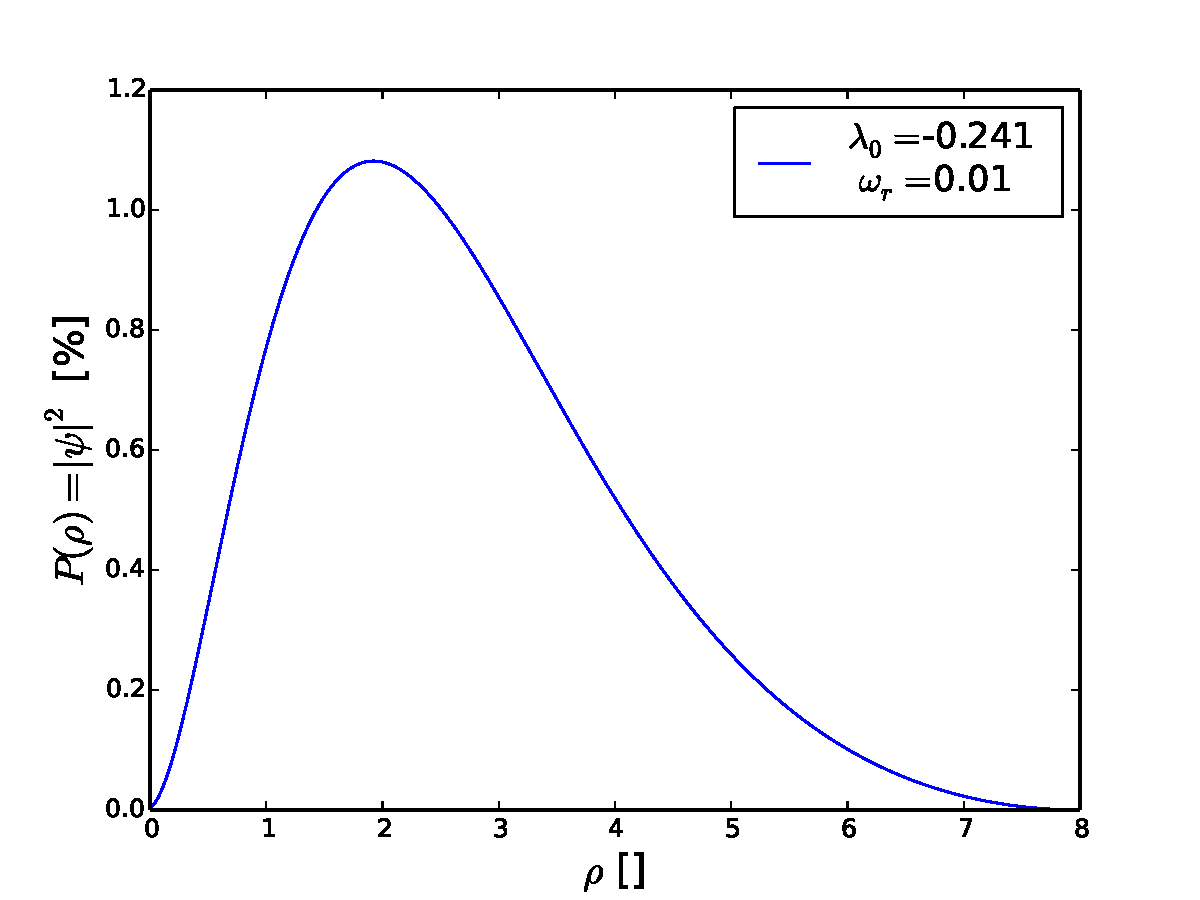
\includegraphics[width=1.1\textwidth]{plot-twoElectrons_01}
				\end{subfigure}
				~ %add desired spacing between images, e. g. ~, \quad, \qquad, \hfill etc
				\begin{subfigure}[b]{0.45\textwidth}
					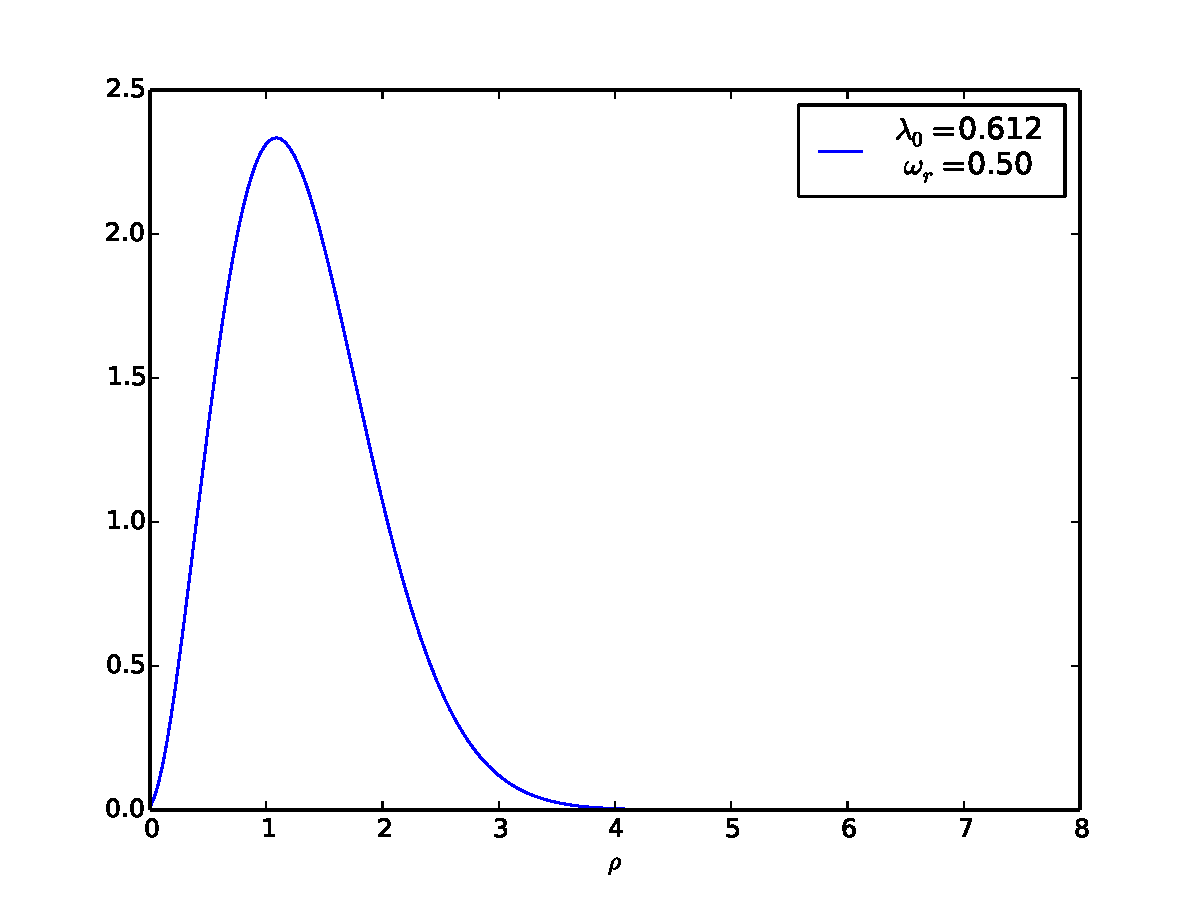
\includegraphics[width=1.1\textwidth]{plot-twoElectrons_05}
				\end{subfigure}
				\begin{subfigure}[b]{0.45\textwidth}
					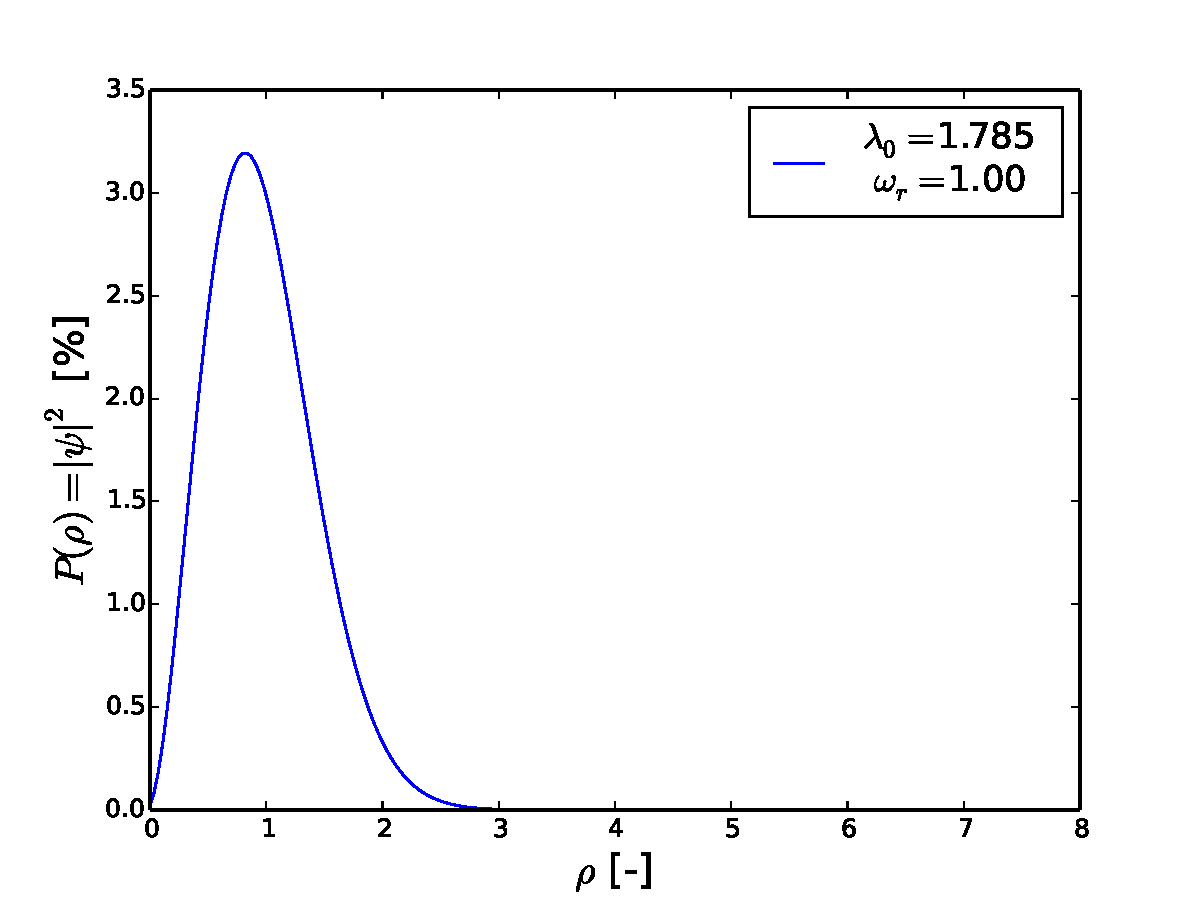
\includegraphics[width=1.1\textwidth]{plot-twoElectrons_1}
				\end{subfigure}
				~ %add desired spacing between images, e. g. ~, \quad, \qquad, \hfill etc
				\begin{subfigure}[b]{0.45\textwidth}
					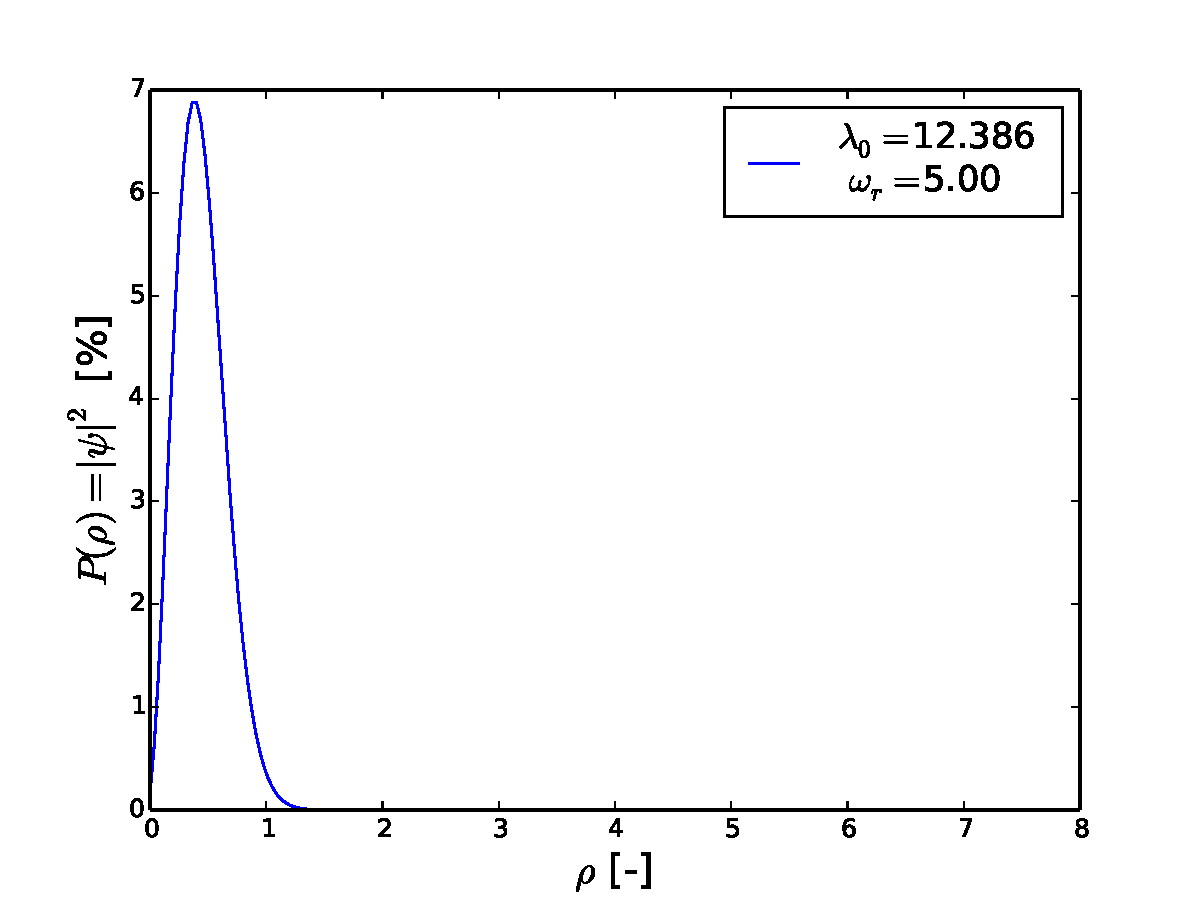
\includegraphics[width=1.1\textwidth]{plot-twoElectrons_5}
				\end{subfigure}
				\caption{Plot of the probability distributions for two electrons with four different oscillator "frequencies" $\omega_r$. }\label{fig: plot two electrons}
			\end{figure}
			
			As the plot show, the oscillator frequency greatly influences the probability distribution of the position of the center of mass for the electron pair, higher frequencies leading to a narrower distribution, much closer to the origin. One other thing to note is that higher frequency leads to larger eigenvalue. This makes direct sense, as the eigenvalues $\lambda\propto E$, and higher frequencies give higher energies. Note also that for $\omega_r=0.01$, we have $\lambda_0<0 \Rightarrow E_0<0$. What this means, I do not have the competence to answer with certainty, however, I propose that this leads to an improper eigenstates (that it is a solution to the \SL equation, however not the normalization condition) and that the ground state in this case is the first to have positive energy. 

		\subsection{Different methods}
			The Jacobi method for finding eigenvalues and eigenvectors is intrinsically slow. Table~\ref{table: tomputation times jacobi vs. numpy} shows the time needed to find the eigenvalues and eigenvectors of the implemented Jacobi method vs. the function \texttt{numpy.linalg.eig} in the python \texttt{numpy} library. Ideally this comparison should be done with a C++ library, e.g. armadillo, but due to a premature system update, this library is not working on my computer. It is to say that the \texttt{numpy.linalg}-library relies heavily on the LAPACK and BLAS libraries, which is also a dependency on armadillo.
			\begin{table}
				\centering
				\caption{Computation times for the Jacobi method and an eigenvalue method from the numpy library in python averaged over 10 runs for each method for each $n$.}
				\label{table: tomputation times jacobi vs. numpy}
				\begin{tabular}{|c|c|c|}
					\hline
					$n$	&	Jacobi [s]	&	Python [s]	\\ \hline
					100	&	0.009	&	0.172	\\
					150	&	0.025	&	0.903	\\
					200	&	0.059	&	2.793	\\
					250	&	0.132	&	6.564	\\
					300	&	0.233	&	13.607	\\
					350	&	0.367	&	24.354	\\
					400	&	0.540	&	40.842	\\ \hline
				\end{tabular}
			\end{table}
			
			As table~\ref{table: tomputation times jacobi vs. numpy} shows, the method in the \texttt{numpy} library is much faster than the implemented Jacobi algorithm. The values for eigenvectors are not, however significantly different for a particular choice of $n$ and $\rho_\mathrm{max}$, meaning for a relatively small system as the one looked at in this project, the jacobi-method is a "good enough" method when it comes to time consummation. 
		
	\section{Conclusion}
		The Jacobi method is a very slow method of finding eigenvalues compared to many other with computation times for a $400\times400$ matrix being around 40 s, compared to 0.5 s for the method embedded in the python \texttt{numpy} llibrary. On average, it is needed around $O(n^2)$ Jacobi rotations to find the eigenvalues of an $n\times n$ matrix, each rotation using around 30-40$n$ FLOPS, leading to $\sim O(n^3)$ FLOPS. 
		
		We have seen that both methods reaches convergence for the three lowest eigenvalues relatively quickly at $n\approx 200$. A good reason to use the Jacobi method that is easily parallelizable, so for systems where a relatively small number of grid points $n$ is sufficient, the Jacobi method may be the preferred method.
		
	
\end{document}



































